\documentclass{beamer}

\usepackage[french]{babel}
\usepackage[T1]{fontenc}
\usepackage[utf8]{inputenc}

\usetheme{Warsaw}
\useoutertheme{infolines}

\usepackage{amsmath}
\usepackage{amssymb}
\usepackage{amsthm}
\usepackage{stmaryrd}

\usepackage{listings}
\usepackage{color}

\definecolor{mygreen}{rgb}{0,0.6,0}
\definecolor{mygray}{rgb}{0.5,0.5,0.5}
\definecolor{mymauve}{rgb}{0.58,0,0.82}

\lstset{ %
  backgroundcolor=\color{white},   % choose the background color
  basicstyle=\footnotesize,        % size of fonts used for the code
  breaklines=true,                 % automatic line breaking only at whitespace
  captionpos=b,                    % sets the caption-position to bottom
  commentstyle=\color{mygreen},    % comment style
  escapeinside={\%*}{*)},          % if you want to add LaTeX within your code
  keywordstyle=\color{blue},       % keyword style
  stringstyle=\color{mymauve},     % string literal style
}

\lstset{language=java} 

\usepackage[all]{xy}

%Les sous listes on des triangles
\setbeamertemplate{itemize item}[circle]
\setbeamertemplate{itemize subitem}[triangle]
%Les elements caché sont grisé
\beamertemplatetransparentcovered

\begin{document}

\title{Android - Fragments, et App Bars}
\author{Jérémy S. Cochoy}
\institute{INRIA Paris-Saclay | jeremy.cochoy@gmail.com}
\date{Mars 2017}


\begin{frame}
\titlepage
\end{frame}

\begin{frame}
  \begin{columns}[t]
  \begin{column}{5cm}
  \tableofcontents[sections={1-3}]
  \end{column}
  \begin{column}{5cm}
  \tableofcontents[sections={4-8}]
  \end{column}
  \end{columns}
\end{frame}

\begin{frame}
\frametitle{La documentation}

\begin{block}{Votre nouveau livre de chevet.}
\begin{center}
\emph{https://developer.android.com/guide/index.html}
\end{center}
\end{block}

\end{frame}

\section{MVC}

\begin{frame}
\frametitle{Le pattern MVC}
\begin{center}
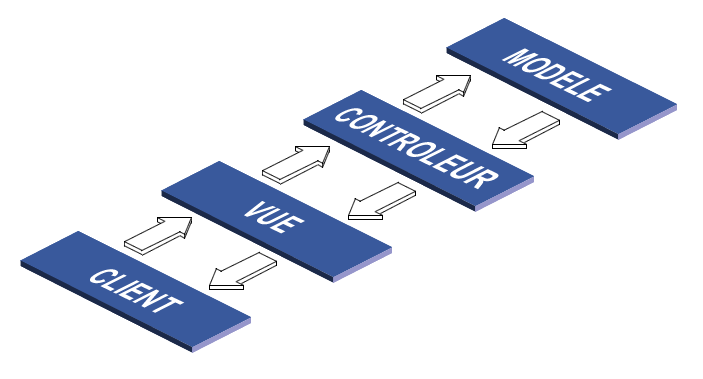
\includegraphics[scale=0.4]{mvc_intro.png}
\end{center}
\end{frame}

\subsection{Vue}
\begin{frame}
\begin{center}

\includegraphics[scale=0.4]{view.png}
\end{center}
\begin{block}{La vue}
C'est l'interface qu'affiche votre application. Dans un projet Android, il s'agit du XML, ainsi que des composants que vous ajoutez dynamiquement via le code de votre activité.
\end{block}
\end{frame}

\subsection{Modèle}
\begin{frame}
\begin{center}

\includegraphics[scale=0.2]{data.jpeg}
\end{center}
\begin{block}{Le modèle}
Une ou des classes qui gèrent l'accès à vos données. Elles peuvent provenir d'un accès distant, un serveur ftp, un fichier local, une base de données locale (SQLite) ou distante (MySQL)...
\end{block}
\end{frame}

\subsection{Contrôleur}
\begin{frame}
\begin{center}

\includegraphics[scale=0.2]{controler.jpeg}
\end{center}
\begin{block}{Le contrôleur}
C'est essentiellement le code de vos activités : le code formate les données, et les envoie dans la vue. Le code gère les actions de l'utilisateur et réagit en conséquence (appel d'une nouvelle activité pour changer la vue, prise de photo, changement des images affichées...).
\end{block}
\end{frame}

\subsection{Intérêt ?}

\begin{frame}
\frametitle{Résumé}
\begin{center}
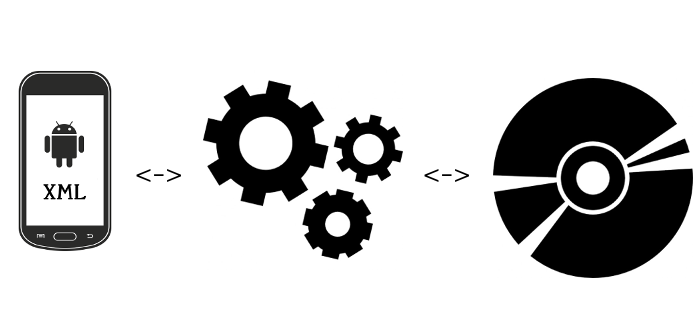
\includegraphics[scale=0.35]{MVC.png}
\end{center}
\begin{block}{Modèle MVC :}
\begin{itemize}
\item Modèle (Model) : Ce qu'on veut afficher.
\item Vue (View) : Comment l'afficher.
\item Contrôleur (Controler) : Formate les données pour les afficher et gère les événements tels que les entrées utilisateur.
\end{itemize}
\end{block}
\end{frame}


\begin{frame}
\frametitle{Avantages du MVC?}
\begin{block}{Indépendance}
Les 3 blocs sont indépendants et communiquent via une interface claire et précise.
\end{block}
\pause
\begin{block}{Substitution du modèle}
Il est possible de remplacer un modèle "fichier local" par un modèle "base de données distante", avec un minimum de modification du code, et sans modification de la vue.
\end{block}
\pause
\begin{block}{Substitution de la vue}
En modifiant uniquement l'XML, on peut revoir le design de l'interface.
\end{block}
\pause
\begin{alertblock}{Dark side}
Attention aux fausses bonnes idées...
\end{alertblock}
\end{frame}



\section{Fragments}

\subsection{Kézako}
\begin{frame}
\frametitle{Les fragments}

\begin{center}

\includegraphics[scale=0.165]{fragments_glass.jpg}
\end{center}

\begin{block}{}
\begin{center}
\verb!FragmentActivity!
\end{center}
\end{block}
\end{frame}

\begin{frame}
\frametitle{Fragments}
\begin{block}{Qu'est-ce qu'un fragment?}
C'est une partie modulaire d'une activité.
\end{block}

\begin{center}
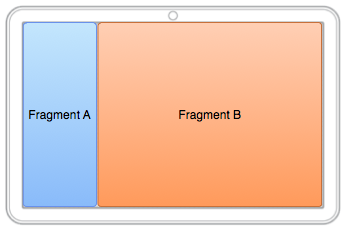
\includegraphics[scale=0.5]{fragments-screen-tab.png}
\end{center}
\end{frame}

\begin{frame}
\frametitle{Fragments}

\begin{block}{Pourquoi utiliser des fragments ?}
Pour permettre à nos applications de s'adapter aux supports physiques.
\end{block}

\begin{center}
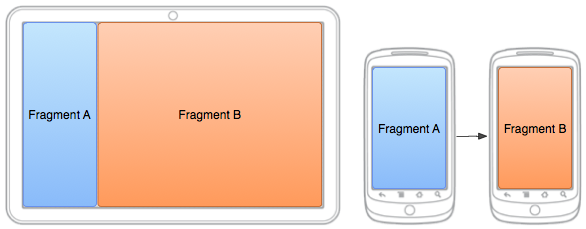
\includegraphics[scale=0.5]{fragments-screen-mock.png}
\end{center}
\end{frame}

\subsection{Créer un fragment}

\begin{frame}
\frametitle{Créer un fragment}
\begin{block}{Comment faire?}
Comme une Activité.
\end{block}

\begin{block}{Une subtilité :}
C'est la méthode \verb!onCreateView()! que l'on redéfinit, et non \verb!onCreate()!.
\end{block}
\end{frame}


\begin{frame}[fragile]
\frametitle{Un fragment vide}
\begin{block}{Code pour créer un fragment}
\lstset{language=java}
\begin{lstlisting}
import android.os.Bundle;
import android.support.v4.app.Fragment;
import android.view.LayoutInflater;
import android.view.ViewGroup;

public class ArticleFragment extends Fragment {
    @Override
    public View onCreateView(LayoutInflater inflater, ViewGroup container,
        Bundle savedInstanceState) {
        // Inflate the layout for this fragment
        return inflater.inflate(R.layout.article_view, container, false);
    }
}
\end{lstlisting}
\end{block}
\end{frame}

\subsection{L'utiliser dans une vue}

\begin{frame}
\frametitle{Ajouter un fragment à son activité}
\begin{block}{Ajouter un fragment via XML}
On peut ajouter du code XML dans layout-large, et un autre dans layout.
\end{block}
\begin{center}

\includegraphics[scale=0.05]{xml-file.png}
\end{center}
\begin{block}{Ajouter un fragment via l'API}
A l'exécution, on peut déterminer la résolution de l'écran et remodeler dynamiquement l'interface.
\end{block}
\begin{center}

\includegraphics[scale=0.05]{api.png}
\end{center}
\end{frame}

\begin{frame}[fragile]
\frametitle{Ajouter un fragment via XML}
\begin{block}{Code pour ajouter deux fragments}
\lstset{language=xml}
\begin{lstlisting}
<LinearLayout ...>
    <fragment android:name="com.example.android.fragments.HeadlinesFragment"
              android:id="@+id/headlines_fragment"
              android:layout_weight="1"
              android:layout_width="0dp"
              android:layout_height="match_parent" />

    <fragment android:name="com.example.android.fragments.ArticleFragment"
              android:id="@+id/article_fragment"
              android:layout_weight="2"
              android:layout_width="0dp"
              android:layout_height="match_parent" />

</LinearLayout>

\end{lstlisting}
\end{block}
\end{frame}

\subsection{UI dynamiques}

\begin{frame}[fragile]
\frametitle{Ajouter un fragment à l'exécution}

\begin{block}{\verb!FragmentManager!}
Il nous faut un gestionnaire de fragment (\verb!FragmentManager!) pour construire un \verb!FragmentTansaction! qui, lui, pourra ajouter / supprimer / remplacer des fragments dans notre activité.
\end{block}
\pause
\begin{alertblock}{Il faut un container}
Il faut un container de type \verb!View! pour y placer nos fragments. Un simple
\lstset{language=xml}
\begin{lstlisting}
<FrameLayout xmlns:android="http://schemas.android.com/apk/res/android"
    android:id="@+id/fragment_container"
    android:layout_width="match_parent"
    android:layout_height="match_parent" />
\end{lstlisting}
    convient.
\end{alertblock}
\end{frame}





\begin{frame}[fragile]
\frametitle{Ajouter un fragment à l'exécution}
\begin{block}{}
Dans \verb!onCreate!, on ajoute un fragment de la façon suivante :
\end{block}
\lstset{language=java}
\begin{lstlisting}
// On verifie qu'on trouve bien notre container.
if (findViewById(R.id.fragment_container) != null) {
// On verifie que c'est le premier lancement de l'activite.
if (savedInstanceState != null) {
  return;
}
// On cree le fragment a placer.
HeadlinesFragment firstFragment = new HeadlinesFragment();          
// On transmet d'eventuels arguments.
firstFragment.setArguments(getIntent().getExtras());         
// On ajoute le fragment au FrameLayout 'fragment_container'.
getSupportFragmentManager().beginTransaction()
    .add(R.id.fragment_container, firstFragment).commit();
}
\end{lstlisting}
\end{frame}

\begin{frame}[fragile]
\frametitle{Ajouter un fragment à l'exécution}

\begin{block}{Détail de la transaction :}
\begin{lstlisting}
//Recuperation du manager
FragmentManager manager = getSupportFragmentManager();

//Creation de la transaction
FragmentTransaction transaction = manager.beginTransaction();
//On ajoute un/des fragments
transaction.add(R.id.fragment_container, firstFragment)
//On 'commit' les operations
transaction.commit();
\end{lstlisting}
\end{block}
\begin{exampleblock}{}
Parce que son ajout est dynamique, ce fragment pourra être retiré ou remplacé.
\end{exampleblock}
\end{frame}


\begin{frame}
\frametitle{Remplacer un fragment}

\begin{block}{Comment remplacer un fragment?}
Avec la méthode \verb!replace()! au lieu de \verb!add()!.
\end{block}
\pause
\begin{block}{Récupérer le fragment remplacé}
Souvent, on souhaite permettre à l'utilisateur "d'annuler"
la transaction et récupérer le fragment précédent.
Pour ça, il suffit d'appeler \verb!addToBackStack()! durant
la transaction.
\end{block}
\pause
\begin{block}{Vie d'un fragment}
Si un fragment est poussé sur la pile de retour, alors il est \emph{stoppé}. Après un retour en arrière, il passera dans l'état \emph{redémarré}. Sinon, il est \emph{détruit}.
\end{block}

\end{frame}

\begin{frame}[fragile]
\frametitle{Remplacer un fragment}

\begin{exampleblock}{Création d'un nouveau fragment et de ses arguments :}
\begin{lstlisting}
//Le fragment
ArticleFragment newFragment = new ArticleFragment();

//Les arguments
Bundle args = new Bundle();
args.putInt(ArticleFragment.ARG_POSITION, position);
newFragment.setArguments(args);
\end{lstlisting}
\end{exampleblock}

\end{frame}
\begin{frame}[fragile]
\frametitle{Remplacer un fragment}

\begin{exampleblock}{Création d'un nouveau fragment}
\begin{lstlisting}
// Commence une transaction
FragmentTransaction transaction = getSupportFragmentManager().beginTransaction();
// Remplace le fragment
transaction.replace(R.id.fragment_container, newFragment);
// Conserve le fragment precedant
transaction.addToBackStack(null);
// Effectue la transaction
transaction.commit();
\end{lstlisting}
\end{exampleblock}


\begin{block}{\verb!addToBackStack()!}
\verb!addToBackStack()! prend en argument une chaîne de caractères optionnelle qui permet de donner un identifiant unique à la transaction, pour effectuer des opérations avancées.
\end{block}

\end{frame}


\subsection{Communication entre fragments}

\begin{frame}
\frametitle{Communiquer entre fragments}
\begin{block}{Comment ?}
La communication se fait via l'activité en lui imposant d'implémenter une \emph{interface}.
\end{block}
\pause
\begin{block}{}
On récupère un pointeur vers l'activité que l'on downcast vers notre interface. Il y a donc un certain nombre de précautions à prendre.
\end{block}
\end{frame}

\begin{frame}
  \begin{block}{Disons que notre fragment hérite de ListFragment...}
    \begin{center}
      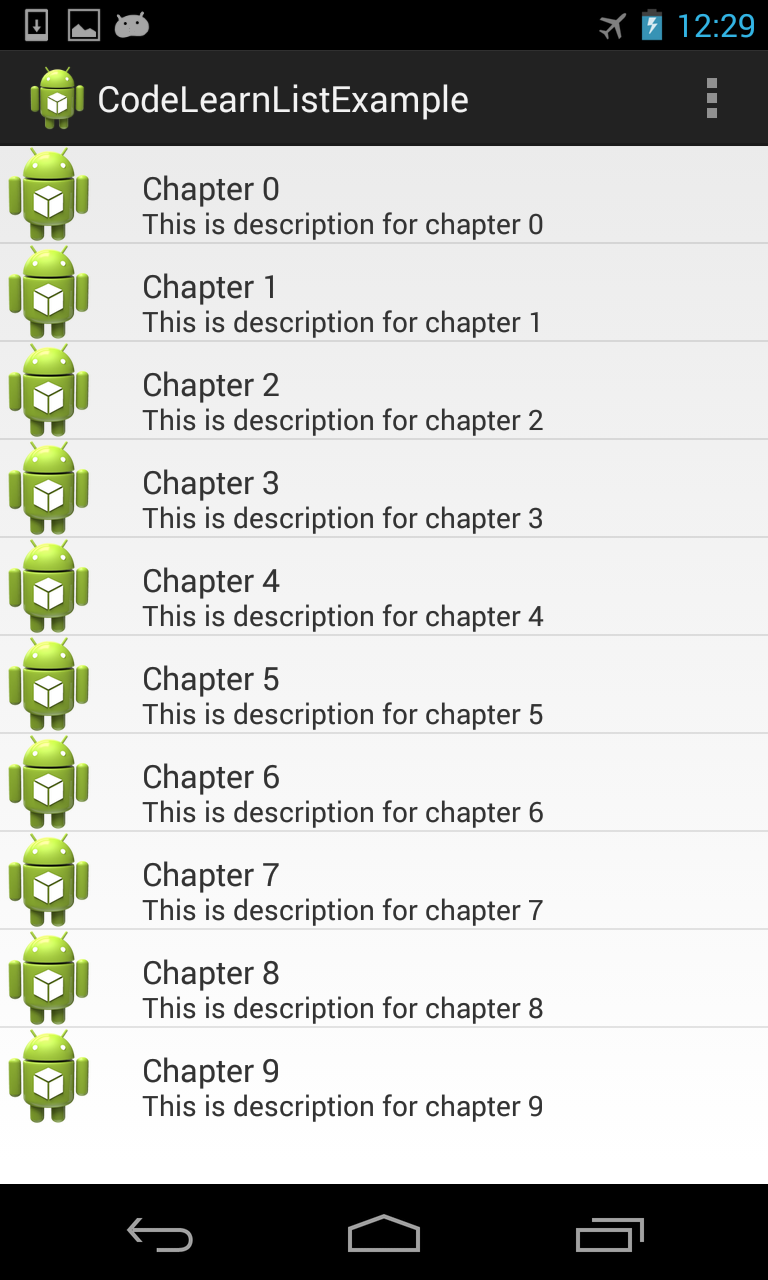
\includegraphics[scale=0.15]{listview.png}
    \end{center}
  \end{block}
\end{frame}

\begin{frame}[fragile]
\frametitle{Forcer une interface pour notre activité}
\begin{block}{On définit notre interface ...}
\begin{lstlisting}
// Notre fragment
public class HeadlinesFragment extends ListFragment {
	// Variable global qui contiendra un pointeur vers l'Activity
    OnHeadlineSelectedListener mCallback;

    // L'Activity contenant le fragment devra implementer l'interface :
    public interface OnHeadlineSelectedListener {
        public void onArticleSelected(int position);
    }
    
    ...
}
\end{lstlisting}
\end{block}
\end{frame}


\begin{frame}[fragile]
\frametitle{Forcer une interface pour notre activité}
\begin{block}{... puis on récupère un pointeur vers l'activité, et on s'assure qu'elle implémente bien notre interface.}
\begin{lstlisting}
  @Override
  public void onAttach(Activity activity) {
    super.onAttach(activity);
        
    // Pour etre sur de la presence d'une implementation,
    // on effectue une conversion explicite vers OnHeadlineSelectedListener.
    try {
      mCallback = (OnHeadlineSelectedListener) activity;
    } catch (ClassCastException e) {
      throw new ClassCastException(activity.toString()
          + " must implement OnHeadlineSelectedListener");
    }
  }
\end{lstlisting}
\end{block}
\end{frame}
    
\begin{frame}[fragile]
\frametitle{Exemple de communication}
\begin{exampleblock}{Un exemple d'utilisation de l'interface :}
\begin{lstlisting}
@Override
    public void onListItemClick(ListView l, View v, int position, long id) {
        // Appelle la fonction de l'Activity.
        mCallback.onArticleSelected(position);
    }
\end{lstlisting}
\end{exampleblock}
\end{frame}

\begin{frame}[fragile]
\frametitle{Coté activité...}
\begin{block}{Implémentation de l'interface}
\begin{lstlisting}
public static class MainActivity extends Activity
        implements HeadlinesFragment.OnHeadlineSelectedListener{
    ...
    
    public void onArticleSelected(int position) {
        // L'utilisateur a choisi un item dans la liste
        // On effectue le necessaire pour afficher l'article correspondant.
    }
}
\end{lstlisting}

\end{block}
\end{frame}

\begin{frame}[fragile]
\frametitle{Pour gérer un mode tablette et un mode mobile...}
\begin{block}{L'activité qui parlait à l'oreille des fragments...}
\begin{lstlisting}
public void onArticleSelected(int position) {

//On cherche notre fragment
  ArticleFragment articleFrag = (ArticleFragment)
    getSupportFragmentManager().findFragmentById(R.id.article_fragment);

  if (articleFrag != null) {
  // On a bien notre fragment, donc on change l'affichage
  articleFrag.updateArticleView(position);
  } else {
    // Suite au prochain slide...
  }
}
\end{lstlisting}
\end{block}
\end{frame}

\begin{frame}
\frametitle{La configuration correspondante}
\begin{center}
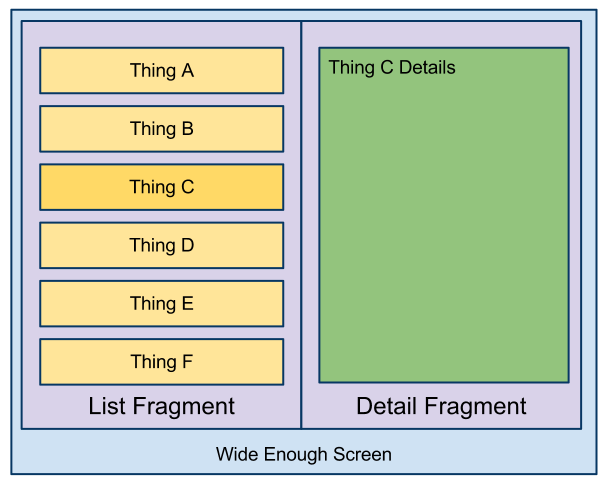
\includegraphics[scale=0.3]{fragments_duo.png}
\end{center}
\end{frame}

\begin{frame}[fragile]
\frametitle{Cas mono-screen...}
\begin{lstlisting}
} else {
  // On est en mode 'un seul ecran'.

  // On construit le nouveau fragment
  ArticleFragment newFragment = new ArticleFragment();
  Bundle args = new Bundle();
  args.putInt(ArticleFragment.ARG_POSITION, position);
  newFragment.setArguments(args);

  //Et on effectue la transaction...
  FragmentTransaction transaction = getSupportFragmentManager().beginTransaction();

  transaction.replace(R.id.fragment_container, newFragment);
  transaction.addToBackStack(null);

  //On realise la transaction
  transaction.commit();
}
\end{lstlisting}
\end{frame}


\begin{frame}
\frametitle{La configuration correspondante}
\begin{center}
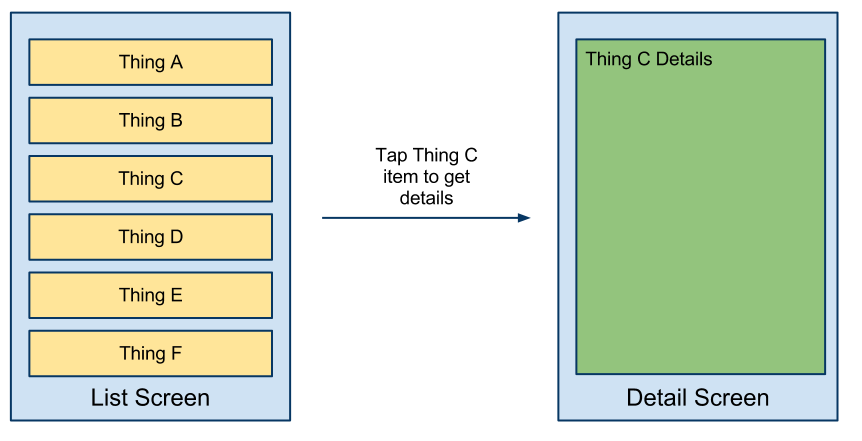
\includegraphics[scale=0.3]{fragments_mono.png}
\end{center}
\end{frame}

\begin{frame}
\frametitle{Cycle de vie d'un fragment}
\begin{center}
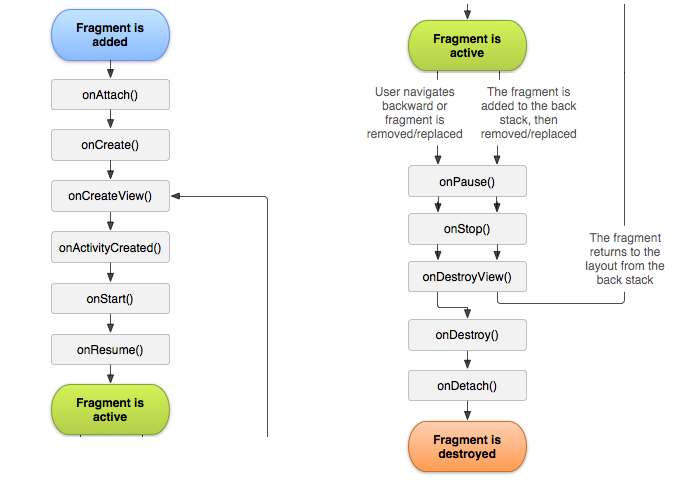
\includegraphics[scale=0.4]{fragment_lifecycle.png}
\end{center}
\end{frame}

\section{App Bar}

\begin{frame}
\frametitle{Qu'est-ce qu'une barre d'application?}

  \begin{center}
  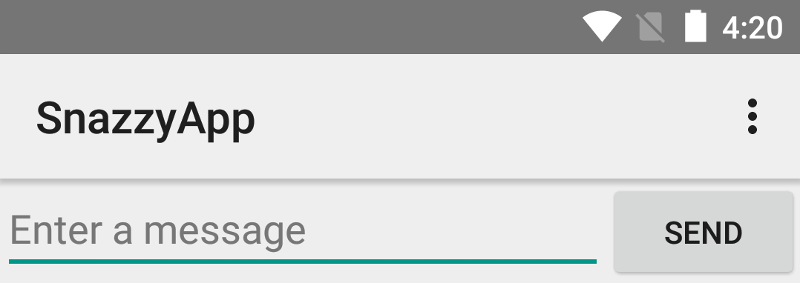
\includegraphics[scale=0.4]{appbar_basic.png}
  \end{center}
\end{frame}

\subsection{Ajouter une App Bar}


\begin{frame}[fragile]
\frametitle{Comment ajouter une ToolBar?}

\begin{block}{Il faut le support de la fonctionnalité.}
Pour ça, il vous faut éventuellement installer la bibliothèque v7 appcompat, si ce n'est pas déjà fait.
\end{block}
\pause
\begin{block}{Et hériter de la bonne classe Activity.}
\begin{lstlisting}
public class MyActivity extends AppCompatActivity {
  // ...
}
\end{lstlisting}

\end{block}
\end{frame}

\begin{frame}[fragile]
\frametitle{Comment ajouter une ToolBar?}

\begin{block}{Il faut le support de la fonctionnalité.}
Pour ça, il vous faut éventuellement installer la bibliothèque v7 appcompat, si ce n'est pas déjà fait.
\end{block}

\begin{block}{Et hériter de la bonne classe Activity.}
\begin{lstlisting}
public class MyActivity extends AppCompatActivity {
  // ...
}
\end{lstlisting}
\pause
\begin{block}{Et choisissez le bon thème.}
\lstset{language=xml}
\begin{lstlisting}
<application
    android:theme="@style/Theme.AppCompat.Light.NoActionBar"
    />
\end{lstlisting}
\lstset{language=java}
\end{block}
\end{block}
\end{frame}


\begin{frame}[fragile]
\frametitle{Comment ajouter une ToolBar?}

\begin{block}{On ajoute la ToolBar à la vue :}
\lstset{language=xml}
\begin{lstlisting}
<android.support.v7.widget.Toolbar
   android:id="@+id/my_toolbar"
   android:layout_width="match_parent"
   android:layout_height="?attr/actionBarSize"
   android:background="?attr/colorPrimary"
   android:elevation="4dp"
   android:theme="@style/ThemeOverlay.AppCompat.ActionBar"
   app:popupTheme="@style/ThemeOverlay.AppCompat.Light"/>
\end{lstlisting}
\lstset{language=java}
\end{block}
\begin{block}{}
Comme c'est une barre d'application, on veut la positionner en haut de l'application.
\end{block}
\end{frame}

\begin{frame}[fragile]
\frametitle{Comment ajouter une ToolBar?}

\begin{block}{On lie la ToolBar au niveau de l'activité :}
\lstset{language=java}
\begin{lstlisting}
@Override
protected void onCreate(Bundle savedInstanceState) {
    super.onCreate(savedInstanceState);
    setContentView(R.layout.activity_my);
    Toolbar myToolbar = (Toolbar) findViewById(R.id.my_toolbar);
    setSupportActionBar(myToolbar);
    }
\end{lstlisting}
\lstset{language=java}
\end{block}
\begin{exampleblock}{Contenu de la barre :}
Par défaut, on y trouve le titre de l'application et un menu déroulant avec pour seul élément "Settings".
\end{exampleblock}
\end{frame}

\subsection{Configurer son AppBar}

\begin{frame}
\frametitle{Personnalisez votre AppBar}
\begin{block}{Une vue XML}
  Les boutons et autres objets sont stockés dans une vue, dans \verb!res/menu!.
\end{block}
\pause
\begin{block}{Ajouter un bouton}
  Pour chaque élément à ajouter, on place un élément \verb!item!.
\end{block}
\pause
\begin{block}{Ce que l'on veut :}
  \begin{center}
  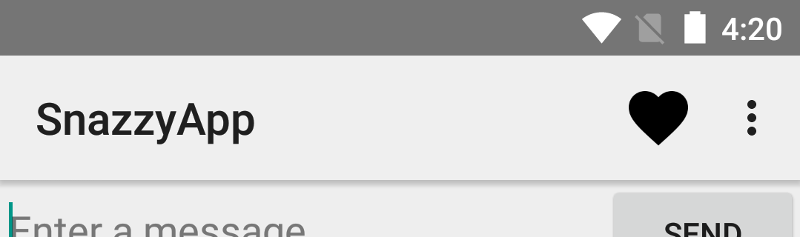
\includegraphics[scale=0.2]{appbar_modif.png}
  \end{center}
\end{block}
\end{frame}

\begin{frame}[fragile]
\frametitle{Personnalisez votre AppBar}
\begin{exampleblock}{Exemple d'AppBar}
\lstset{language=xml}
\begin{lstlisting}
<menu xmlns:android="http://schemas.android.com/apk/res/android" >
    <!-- Si possible, "Mark Favorite", doit apparaitre comme un bouton. -->
    <item
        android:id="@+id/action_favorite"
        android:icon="@drawable/ic_favorite_black_48dp"
        android:title="@string/action_favorite"
        app:showAsAction="ifRoom"/>

    <!-- Configuration doit Toujours etre dans le menu deroulant. -->
    <item android:id="@+id/action_settings"
          android:title="@string/action_settings"
          app:showAsAction="never"/>
</menu>
\end{lstlisting}
\lstset{language=java}
\end{exampleblock}

\end{frame}

\subsection{Réagir aux actions}

\begin{frame}
\frametitle{Comment réagir à un clic ?}
\begin{block}{Au moment où l'utilisateur clique :}
La méthode \verb!onOptionsItemSelected()! est appelé, avec en argument un \verb!MenuItem! correspondant à l'item cliqué. La méthode \verb!MenuItem.getItemId()! permet de récupérer l'ID de l'élément.
\end{block}
\end{frame}

\begin{frame}[fragile]
\begin{block}{Retrouvons notre exemple :}
\lstset{language=java}
\begin{lstlisting}
@Override
public boolean onOptionsItemSelected(MenuItem item) {
    switch (item.getItemId()) {
        case R.id.action_settings:
            // Lancer l'Activity "configuration".
            return true;

        case R.id.action_favorite:
            // Ajouter l'article courant aux favoris
            return true;

        default:
            // Action non reconnue, dans le doute on laisse faire la classe parente.
            return super.onOptionsItemSelected(item);
    }
}
\end{lstlisting}
\end{block}

\end{frame}

\begin{frame}
\begin{center}
Pour me contacter : jeremy.cochoy@gmail.com, merci et à bientôt.

\medskip
\medskip
\medskip
\medskip


\includegraphics[scale=0.18]{android.jpg}
\end{center}
\end{frame}




\end{document}